\section{Definiera skärningstal}\par
\noindent Detta är slutklämmen på kursen, vi vill definiera skärningstalet och bevisa att den upfyller axiomen.
\par\bigskip
\noindent\textbf{Anmärkning:}\par
\noindent Koordinatringen för $\C^2$ är $\C[x,y]$ (ringen av reguljära funktioner på $\C^2$) (är en $c$-algebra)
\par\bigskip
\noindent\textbf{Anmärkning:}\par
\noindent Viktigt ideal är $(f)$ där $f$ är ett polynom, motsvarar ($\Lrarr$) $V(f)$.\par
\noindent Ännu viktigare är idealet som hör till en punkt (maximala idealet); motsvarar punkter $P=(a,b)\in\C^2\Rightarrow m = (x-a,y-b)$ (här är paranteserna idealet, och inte beteckningen för en punkt)\par
\noindent Ett sätt att visa att det är ett maximalt ideal är att kvota med $\C[x,y]$, vi får då en kropp och det finns en sats som säger att om vi kvotar med ett ideal och får en kropp så är det ett maximalt ideal.\par
\noindent Ett annat sätt att se det på är:
\begin{equation*}
  \begin{gathered}
    m = \left\{f\in\C[x,y]|f(a,b) = 0\right\} = \left\{f\in\C[x,y]|\text{$f$ har ingen konstantterm då $f$ T.U kring $a,b$}\right\}
  \end{gathered}
\end{equation*}
\par\bigskip
\noindent\textbf{Anmärkning:}\par
\noindent Lokalisering handlar om att vi vill invertera \textit{vissa} element.
\par\bigskip
\noindent Vi kommer att lokalisera endast i $S = R\backslash m$ (vi kommer alltid kunna göra detta om $m$ är primideal, vilket $m$ är om det är maximalt) och $R$ är en polynomring i 1 eller 2 variabler (vi kör på 2).
\par\bigskip
\begin{theo}
  OOm $R$ integritetsområde och $S$ är en multiplikativ mängd $S\subseteq R$, då är\par
  \begin{itemize}
    \item $S^{-1}R$ ett integritetsområde
    \item $R\to S^{-1}R$ $r\mapsto r/1$ är injektiv
  \end{itemize}
\end{theo}
\par\bigskip
\begin{theo}
  O$\mathcal{O}_p$ har exakt ett maximalt ideal, nämligen $m\mathcal{O}_p$
\end{theo}
\par\bigskip
\begin{prf}
  ALåt $I$ vara ett ideal så att $m\mathcal{O}_p\subset I$.\par
  \noindent Tag $F\in I\backslash m\mathcal{O}_p$. Det innebär att $F$ är en kvot så att nämnaren inte är 0. Men sådana element är inverterbara.\par
  \noindent Vi har då ett element i $I$ som är inverterbart i $\mathcal{O}$, men då måste $I$ vara hela ringen, så $I = R$ ($F(p)\neq0$)
  \par\bigskip
  \noindent Ungefär samma argument visar att $\mathcal{O}_p$ är unikt
\end{prf}
\par\bigskip
\noindent\textbf{Anmärkning:}\par
\noindent $R$ med 1 enda maximalt ideal kallas för en \textit{lokal ring}. Dessa är en viktig klass av ringar. Det finns fler sådana, ringen av formella potensserier exvis.
\par\bigskip
\noindent I allmänhet, så fort man lokaliserar i ett primideal får man en lokal ring ($R_p = $ lokal ring) 
\par\bigskip
\noindent Poängen med $\mathcal{O}_p$ är att den innehåller all väsentlig algebraisk information om geometri nära $p$ (i någon mening).\par
\par\bigskip
\noindent Låt oss titta mer på vad lokalisering gör. Betrakta följande koordinatring för 2 punkter ($x = 0$ och $x=1$) i $\C$.\par
\noindent Det är någon algebraisk mängd, och idealet genereras av polynomet som är produkten av $x$ och $(x-1)$ (det som är 0 i 0 och 0 i 1, allt annat har dessa 2 polynom som faktorer), vi får då:
\begin{equation*}
  \begin{gathered}
    \C[X]/(x(x-1))
  \end{gathered}
\end{equation*}\par
\noindent Notera att detta även är ett radikalt ideal. Det är inte svårt att se att denna är isomorf med ringen $\C^2 = \C$x$\C$:
\begin{equation*}
  \begin{gathered}
    \C[x]/(x(x-1))\to\C^2\\
    f\mapsto (f(0),f(1))
  \end{gathered}
\end{equation*}
\par\bigskip
\noindent Om vi lokaliserar i $x=0$, dvs betrakta $m = (x)$ så får vi ringen $\C[m]_m$\par
\noindent Vi kan betrakta $\C[x]_m/(x(x-1))_m$
\par\bigskip
\noindent Men, då kan vi först observera en sak, och det är att det här idealet $(x(x-1))_m$ är faktiskt samma ideal som $(x)_m$. Anledningen till det är att i ringen $\C[x]_m$ så är $(x-1)$ inverterbart (för $x-1$ är inte 0 i 0):
\begin{equation*}
  \begin{gathered}
    xf(x) = x(x-1)\dfrac{f(x)}{x-1}\text{ i } \C[x]_m
  \end{gathered}
\end{equation*}\par
\noindent Då kan vi föränkla och skriva på följande sätt:
\begin{equation*}
  \begin{gathered}
    \C[x]_m/(x(x-1))_m = \C[x]_m/(x)_m \cong \C
  \end{gathered}
\end{equation*}\par
\noindent Något i $\C[x]_m/(x(x-1))_m$ representeras av:
\begin{equation*}
  \begin{gathered}
    \dfrac{a_0+a_1x+a_2x^2+\cdots}{b_0+b_1x+b_2x^2+\cdots}
  \end{gathered}
\end{equation*}\par
\noindent Detta kan vi skicka till $\dfrac{a_0}{b_0}$ eftersom:
\begin{equation*}
  \begin{gathered}
    \dfrac{a_0+a_1x+a_2x^2+\cdots}{b_0+b_1x+b_2x^2+\cdots} \sim\dfrac{a_0}{b_0}\Lrarr b_0(a_0+a_1x+\cdots)-(b_0+b_1x+\cdots)a_0 = x(\cdots)
  \end{gathered}
\end{equation*}
\newpage
\subsection{Skärningstalet}\hfill\\\par
\noindent Om $f,g$ är 2 polynom i $\C[x,y]$ så generar de ideal $(f,g)\subseteq\C[x,y]_m$ där $m = (x-a,y-b)$. Vi kallar $\C[x,y]_m = \mathcal{O}$
\par\bigskip
\begin{theo}[Skärningstal]{thm:intersectnumb}
  Notera att allt är vektorrum
  \par\bigskip
  \noindent Vi definierar skärningstalet som:
  \begin{equation*}
    \begin{gathered}
      I_p(f,g) = dim_{\C}\left(\mathcal{O}/(f,g)\right)
    \end{gathered}
  \end{equation*}\par
  \noindent Kan även skrivas på:
  \begin{equation*}
    \begin{gathered}
      \mathcal{O}/(f,h)\mathcal{O}_p = \C[x,y]_m/(f,g)_m
    \end{gathered}
  \end{equation*}
\end{theo}
\par\bigskip
\noindent\textbf{Anmärkning:}\par
\noindent Skärningstalet definieras lokalt i en punkt, vi vill inte ha information om saker som sker långt bort.
\par\bigskip
\noindent\textbf{Exempel:}\par
\noindent Låt $p=(0,0)$, titta på $I_{(0,0)}(x,y)$:
\begin{equation*}
  \begin{gathered}
    = \mathcal{O}_{(0,0)}/(x,y)_{(0,0)} = \C \Rightarrow dim_{\C} = 1
  \end{gathered}
\end{equation*}
\par\bigskip
\noindent\textbf{Exempel:}\par
\noindent $I_0(y,y-x^2)$ = $dim_{\C}\left(\mathcal{O}_{(0,0)}/(y,y-x^2)\right)$:
\begin{equation*}
  \begin{gathered}
    \mathcal{O}_{(0,0)}/(y,y-x^2) = \mathcal{O}_{(0,0)}/(y,x^2)\cong \C[x]_m/(x^2)_m\stackrel{c-vektorrum}{\cong}\C^2\\
    \C[x]_m/(x^2)_m = \left(\C[x]/(x^2)\right)_m
  \end{gathered}
\end{equation*}\par
\noindent Vi tittar på något i kvotringen:
\begin{equation*}
  \begin{gathered}
    \dfrac{f}{g}+(x^2)_m\\
    \dfrac{f}{g} = \dfrac{f(0)}{g(0)}+\left(\dfrac{f}{g}\right)^{\prime}(0)x
  \end{gathered}
\end{equation*}\par
\noindent Det som överlever i kvotringen är lijäriseringen av funktioner.
\par\bigskip
\noindent Dimensionen av $\C^2$ är givetvis 2 = $I_0(y,y-x^2)$
\par\bigskip
\noindent\textbf{Anmärkning:}\par
\noindent Till vilken ring som helst kommer det tillhöra en geomtrisk motsvarighet.
\par\bigskip
\noindent\textbf{Exempel:}\par
\noindent Låt $f = y-x^3(x-1)$ och $g = y$, för $f = 0\Lrarr y=x^3(x-1)$ som nära 0 blir $\approx -x^3$ och nära 1 blir den ungefär linjär.\par
\noindent Vi gör liknande räkningar:
\begin{equation*}
  \begin{gathered}
    \C[x,y]_m/(f,g)\cong\C[x]_m/(x^3(x-1))
  \end{gathered}
\end{equation*}\par
\noindent Lokalisera i $m = (x)$, då är $(x-1)$ inverterbart (nollskillt i 0), kvar får vi då:
\begin{equation*}
  \begin{gathered}
    \C[x]_m/(x^3)_m\cong\C^3
  \end{gathered}
\end{equation*}\par
\noindent Lokalisera i $m=(x-1)$, då får vi att $x^3$ är inverterbart och vi får kvar:
\begin{equation*}
  \begin{gathered}
    \C[x]_m/(x-1)_m\cong\C
  \end{gathered}
\end{equation*}
\par\bigskip
\noindent Vi kan för skojs skull titta på den generaliserade koordinatringen:
\begin{equation*}
  \begin{gathered}
    \C[x,y]/(f,g) = \C[x]/(x^3(x-1))\cong\C^4\text{ (4 termer i T.U)}\Rightarrow\C^4 = \C^3\oplus\C
  \end{gathered}
\end{equation*}
\par\bigskip
\begin{theo}
  A$I_p(f,g)$ uppfyller axiomen
\end{theo}
\par\bigskip
\begin{prf}[Axiom 0]{prf:axiom0}
  Hur ser projektiva transformationer ut i affina kartor?
  \begin{equation*}
    \begin{gathered}
      F(x,y,z) = (ax+by+cz,dx+ey+fz,\cdots)
    \end{gathered}
  \end{equation*}\par
  \noindent En projektiv transformation i en karta ser ut på följande:
  \begin{equation*}
    \begin{gathered}
      (x,y)\stackrel{F}{\mapsto} \left(\dfrac{ax+by+c}{gx+hy+k},\dfrac{dx+ey+f}{gx+hy+k}\right)
    \end{gathered}
  \end{equation*}\par
  \noindent Denna är inverterbar. Precis som vanligt, när vi har en affin avbildning så inducerar den en avbildning med polynomringen:
  \begin{equation*}
    \begin{gathered}
      \C[x,y]\stackrel{\cong}{\to}\C[x,y]\qquad f\mapsto f\circ F  =F^*F\\
      \C(x,y)\to\C(x,y)\qquad \dfrac{f}{g}\mapsto \dfrac{f\circ F}{g\circ F}
    \end{gathered}
  \end{equation*}\par
  \noindent Här sammansätter vi funktioner med en annan funktion, då får vi en ny funktion. Denna "operation" är inverterbar, så det finns en isomorfi.
  \par\bigskip
  \noindent Varför vill vi göra så? Jo, vi har avbildningen: (Figure 2)
\end{prf}
  \begin{figure}[ht!]
      \centering
      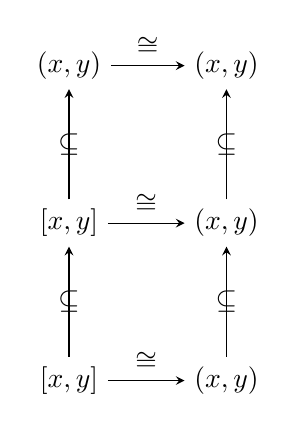
\begin{tikzpicture}
        \node (p0){$\C(x,y)$};
        \node[right of=p0, xshift=1cm](p1){$\C(x,y)$};
        \node[below of=p0, yshift=-1cm](p2){$\C[x,y]$};
        \node[right of=p2, xshift=1cm](p3){$\C(x,y)$};
        \node[below of=p2, yshift=-1cm](p4){$\C[x,y]$};
        \node[right of=p4, xshift=1cm](p5){$\C(x,y)$};
        \path[-stealth] (p0) edge[above] node{$\cong$} (p1);
        \path[-stealth] (p2) edge[above] node{$\cong$} (p3);
        \path[-stealth] (p4) edge[above] node{$\cong$} (p5);
        \path[-stealth] (p2) edge node{$\subseteq$} (p0);
        \path[-stealth] (p3) edge node{$\subseteq$} (p1);
        \path[-stealth] (p4) edge node{$\subseteq$} (p2);
        \path[-stealth] (p5) edge node{$\subseteq$} (p3);
      \end{tikzpicture}
      \caption{}
  \end{figure}
\par\bigskip
\begin{prf}[Axiom 1]{prf:axiom1}
  Vi kan säga att $I_p(f,g) = I_p(g,f)$, detta är uppenbart för idealet som $f,g$ genererar är samma som $g,f$ 
\end{prf}
\par\bigskip
\begin{prf}[Axiom 2]{prf:axiom2}
  \begin{equation*}
    \begin{gathered}
      I_p(f,g) = 0\Lrarr dim_{\C} \C[x,y]_m/(f,g)_m = 0\Lrarr \C[x,y]_m = (f,g)_m = af+bg=1\quad a,b\in\C[x,y]_m
    \end{gathered}
  \end{equation*}\par
  \noindent Från detta följer det att $f,g$ inte båda kan vara 0 i $p$, eftersom $0\neq1$, då har vi:
  \begin{equation*}
    \begin{gathered}
      I_p\neq0 \Rightarrow f,g\neq0
    \end{gathered}
  \end{equation*}
  \par\bigskip
  \noindent Vi visar det omvända. Att $f(p)\neq0$ betyder det att vi kan invertera $f$ i $\mathcal{O}_p$. Men, ett ideal som innehåller ett inverterbart element är hela ringen, och då är $\C[x,y]_m=(f,g)_m\Rightarrow I_p(f,g)=0$
\end{prf}
\par\bigskip
\begin{prf}[Axiom 3]{prf:axiom3}
  För beviset att $I_0(x,y) = 1$, se exempel.
\end{prf}
\par\bigskip
\noindent För att visa 4 behöver vi införa lite verktyg:
\par\bigskip
\begin{theo}[Summa]{thm:sum}
  Låt $V$ vara ett vektorrum och $U, W$ underrum till $V$.
  \par\bigskip
  \noindent Vi säger att $V$ är \textit{summan} av $U,W$ om:
  \begin{equation*}
    \begin{gathered}
      \forall v\in V:\:\exists u\in U,w\in W\; v = u+w
    \end{gathered}
  \end{equation*}\par
\noindent Vi skriver då $V = U+W$. Notera att $U\cap W$ inte nödvändigtvis behöver vara $\left\{0\right\}$ 
\end{theo}
\par\bigskip
\begin{theo}[Direkt summa]{thm:direcftsum}
$V$ kallas \textit{direkta summan} av $U,W$ om $V = U+W$ och $U\cap W = \left\{0\right\}$
\par\bigskip
\noindent Betcknas med $\oplus$
\end{theo}
\par\bigskip
\noindent\textbf{Exempel:}\par
\noindent $F:V\to V$ är diagonaliserbar $\Lrarr V = \bigoplus_{\lambda}V_{\lambda}$ där $V_{\lambda}$ är egenrum till egenvektor $\lambda$
\par\bigskip
\begin{theo}
  EEn följd av linjära rum och linjära avbildningar $U\stackrel{f}{\to}V\stackrel{g}{\to}W$ kallas \textit{exakt vid $V$} om:
  \begin{equation*}
    \begin{gathered}
      ker(g) = im(f)
    \end{gathered}
  \end{equation*}
\end{theo}
\par\bigskip
\begin{theo}
  EEn följd $0\to U\stackrel{f}{\to}V\stackrel{g}{\to}W\to 0$ kallas exakt om den är exakt vid $U,V,W$
  \par\bigskip
  \noindent Notera! $V = U\oplus W$
\end{theo}
\par\bigskip
\begin{theo}
  OOm vi har en exakt följd $0\to U\stackrel{\varphi}{\to}V\stackrel{\psi}{\to}W\to 0$ (kort exakt följd), så gäller att det finns $U^{\prime},W^{\prime}\subset V$  så att:
  \begin{equation*}
    \begin{gathered}
      U^{\prime}\cong U\qquad W^{\prime}\cong W\\
      V = U^{\prime}\oplus W^{\prime}
    \end{gathered}
  \end{equation*}
\end{theo}
\newpage
\begin{prf}
  ADet finns en avbildning $s:W\to V$ som är injektiv och uppfyller att $\psi\circ s = id_W$. \par
  \noindent Nömligen, för varje element $\overline{e_{\alpha}}$ i en bas för $W$, tag $\overline{v_{\alpha}}\in V$ så att $\psi(\overline{v_{\alpha}}) = \overline{e_{\alpha}}$ (detta kan vi göra för att $\psi$ är surjektiv)
  \par\bigskip
  \noindent Definiera $s(\overline{e_{\alpha}}) = \overline{v_{\alpha}}$ (här är $s$ unikt bestämd av detta).\par
  \noindent Då är $\psi\circ s(\overline{e_{\alpha}}) = \psi(\overline{v_{\alpha}}) = \overline{e_{\alpha}}$
  \par\bigskip
  \noindent Betrakta nu först $\psi$ och sedan $s$, dvs $s\circ\psi\stackrel{def}{=}\Pi$.\par
  \noindent Vi ser direkt att $\Pi^2 = (s\circ\psi)\circ(s\circ\psi) = s\circ\underbrace{(\psi\circ s)}_{\text{$id_W$}}\circ\psi = \Pi$
  \par\bigskip
  \noindent Varje element i $V$ kan skrivas $\overline{v} = (v-\Pi(\overline{v}))+\Pi(\overline{v})$
  \par\bigskip
  \noindent Notera! $\Pi(\overline{v}-\Pi(\overline{v})) = \Pi(\overline{v})-\Pi^2(\overline{v}) =\Pi(\overline{v})-\Pi(\overline{v})=0\Rightarrow \overline{v}-\Pi(\overline{v})\in ker(\Pi)$ och $\Pi(\overline{v})\in im(\Pi)$
  \par\bigskip
  \noindent Eftersom $s$ är injektiv, så dör inget där men saker dör i $\psi$, så $ker(\psi) = ker(\Pi) = im(\varphi)\stackrel{def}{=}U^{\prime}\cong U$ 
  \par\bigskip
  \noindent Då är även $im(\Pi) = im(s) = W^{\prime}\cong W$
  \par\bigskip
  \noindent Vi har nu sätt att $V = U+W$ Vi visar nu att snitter är 0, vilket inte är svårt att se ty $U = im(\varphi)$ och $W=im(s)$, snittet är rimligtvis $\left\{0\right\}$, vi visar detta:
  \par\bigskip
  \noindent Om ett element ligger i $U^{\prime}\cap W^{\prime}$ så kan det skrivas på 2 sätt, nämligen som:
  \begin{equation*}
    \begin{gathered}
      \varphi(\overline{a}) = s(\overline{b})
    \end{gathered}
  \end{equation*}
  \noindent Om vi nu tar $\psi$ på båda led får vi:
  \begin{equation*}
    \begin{gathered}
      \underbrace{\psi\circ\varphi(\overline{a})}_{\text{=0}} = \underbrace{\psi\circ s(\overline{b})}_{\text{$\overline{b}$}}\\
      \Rightarrow\overline{b} = 0\Rightarrow s(\overline{b}) = 0
    \end{gathered}
  \end{equation*}
  \par\bigskip
  \noindent Något vi har visat nu är även $dim V = dim U + dim W$
\end{prf}
\newpage
\begin{prf}[Axiom 4]{prf:axiom4}
  Vi gör detta genom att konstruera en kort exakt följd:
  \begin{equation*}
    \begin{gathered}
      0\to \mathcal{O}_p/(f,h)_m\stackrel{\varphi}{\to}\mathcal{O}_p/(f,gh)_m\stackrel{\psi}{\to}\mathcal{O}_p/(f,g)_m\to0
    \end{gathered}
  \end{equation*}\par
  \noindent Varifrån det följer att $dim V = dim U + dim W$
  \par\bigskip
  \begin{equation*}
    \begin{gathered}
      \Phi(x+(f,h)_m) = g+(f,gh)_m\\
      \psi(z+(f,gh)_m) = z+(f,g)_m
    \end{gathered}
  \end{equation*}
  \par\bigskip
  \noindent Vi vill visa 3 saker:\par
  \begin{itemize}
    \item $\psi$ är surjektiv (uppenbart)
    \item $ker(\psi) = im(\Phi)$
    \item $\Phi$ är injektiv
  \end{itemize}\par
  \noindent Vi visar andra punkten:
  \begin{equation*}
    \begin{gathered}
      z+(f,gh)_m\in ker(\psi)\Lrarr z+(f,g)_m =0\Lrarr z=\alpha f+\beta g = \beta g\\
      z+(f,gh) = \beta g+(f,gh)\in im(\Phi)
    \end{gathered}
  \end{equation*}
  \par\bigskip
  \noindent Vi visar 3dje. Vad betyder det att $\Phi$ är injektiv? Vi måste ta något som går till 0 och visar att ursprunget ligger i idealet:
  \begin{equation*}
    \begin{gathered}
      z +(f,h)_m\in ker(\Phi) \Lrarr\exists a,b\in\mathcal{O}_p: gz = af+bgh
    \end{gathered}
  \end{equation*}
  \par\bigskip
  \noindent Notera att $f,g,h$ är polynom, medan $z,a,b$ har nämnare som alla är nollskillda i $p$
  \par\bigskip
  \noindent Låt $S$ produkten av nämnarna så att $g\underbrace{(Sz)}_{\text{C}} = \underbrace{(aS)}_{\text{A}}f+\underbrace{(bS)}_{\text{B}}gh$\par
  \noindent Då är $g(C-Bh) = Af$
  \par\bigskip
  \noindent\textbf{Fall 1}: $f|(C-Bh)$ så $Df = C-Bh$ för något polynom $D$, men $C = Sz$, vilket ger:
  \begin{equation*}
    \begin{gathered}
      Sz = Df+Bh\Rightarrow z 0 \dfrac{D}{S}f+\dfrac{B}{S}h
    \end{gathered}
  \end{equation*}
  \par\bigskip
  \noindent\textbf{Fall 2}: $f,g$ har gemensam faktor (vi kan anta att den är irreducibel för att underlätta) $q$:\par
  \noindent Vi vill vissa:
  \begin{equation*}
    \begin{gathered}
      dim_{\C} \C[x,y]_m/(f,g)_m = \infty
    \end{gathered}
  \end{equation*}
  \par\bigskip
  \noindent Vi gör det genom en slags jämförelsesats, vi visar att:
  \begin{equation*}
    \begin{gathered}
      \C[x,y]/(p)
    \end{gathered}
  \end{equation*}\par
  \noindent har oändlig dimension ($p$ är en irreducibel kurva).
\end{prf}
\par\bigskip
\begin{prf}[Axiom 5]{prf:axiom5}
  Vi kan säga att $I_p(f,g+hf) = I_p(f,g)$, detta är uppenbart för idealet som $f,g+hf$ genererar är samma som $f,g$ 
\end{prf}
